\chapter{二次接线图分析}
\section{概述}
在牵引变电所和供电装置中,高压开关设备的控制、信号以及主设备监测电路都属于二次接线,它们构成了电气系统的重要组成部分。近年来,随着计算机和大规模集成电路技术的发展,我国轨道交通的牵引变电所二次设备的技术水平发生了巨大变化。目前广泛应用的牵引变电所综合自动化技术将控制、保护、数据采集和监控等功能集成在一起,取代了传统的控制和信号系统,尽管原理仍然与传统的二次接线系统相同。

为确保牵引变电所和供电装置的一次电气设备能够安全可靠且经济地运行,并实现对其进行监测和控制,需要配置完整的二次设备,包括控制、信号、继电保护、自动装置和监测仪表等。二次设备的电气连接关系通常以特定的图形和文字符号表示,称为二次接线图,它是电气系统的重要组成部分。

通常,二次接线图有三种主要表现形式,分别为原理接线图、展开接线图和安装接线图。本课程设计主要采用展开接线图。展开接线图是在相应原理接线图的基础上,将电路分为交流电流、电压回路以及直流回路等相对独立的各个组成部分,并对它们进行分别讨论。在展开接线图中,设备元件的不同线圈和接点等将分别连接到相应部分的电路中。

在展开接线图的直流回路部分,力求按照各部件流通电流的顺序排列,即按其工作时可能的动作顺序,自上而下、由左至右地排列成行。对于相同元件的不同线圈和接点,应使用相同的文字标注,并在展开接线图的一侧可以添加文字说明,以便清晰地理解相应部分电路的功能。

\section{进线柜二次接线图分析}

在城轨供变电技术中,进线柜是供电系统的重要组成部分,其主要功能是引入外部电源并提供控制和保护。它充当了电力系统的入口,用于引入、分配、调整和保护电力。进线柜的功能包括电力引入、电压调整、电力控制、电力监测和测量、电力保护,以及隔离和安全。通过有效的进线柜设计和运营,城轨供电系统能够获得稳定可靠的电力供应,以支持城轨交通的正常运行。

\subsection{进线柜控制信号回路分析}

\begin{figure}[!h]
	\centering
	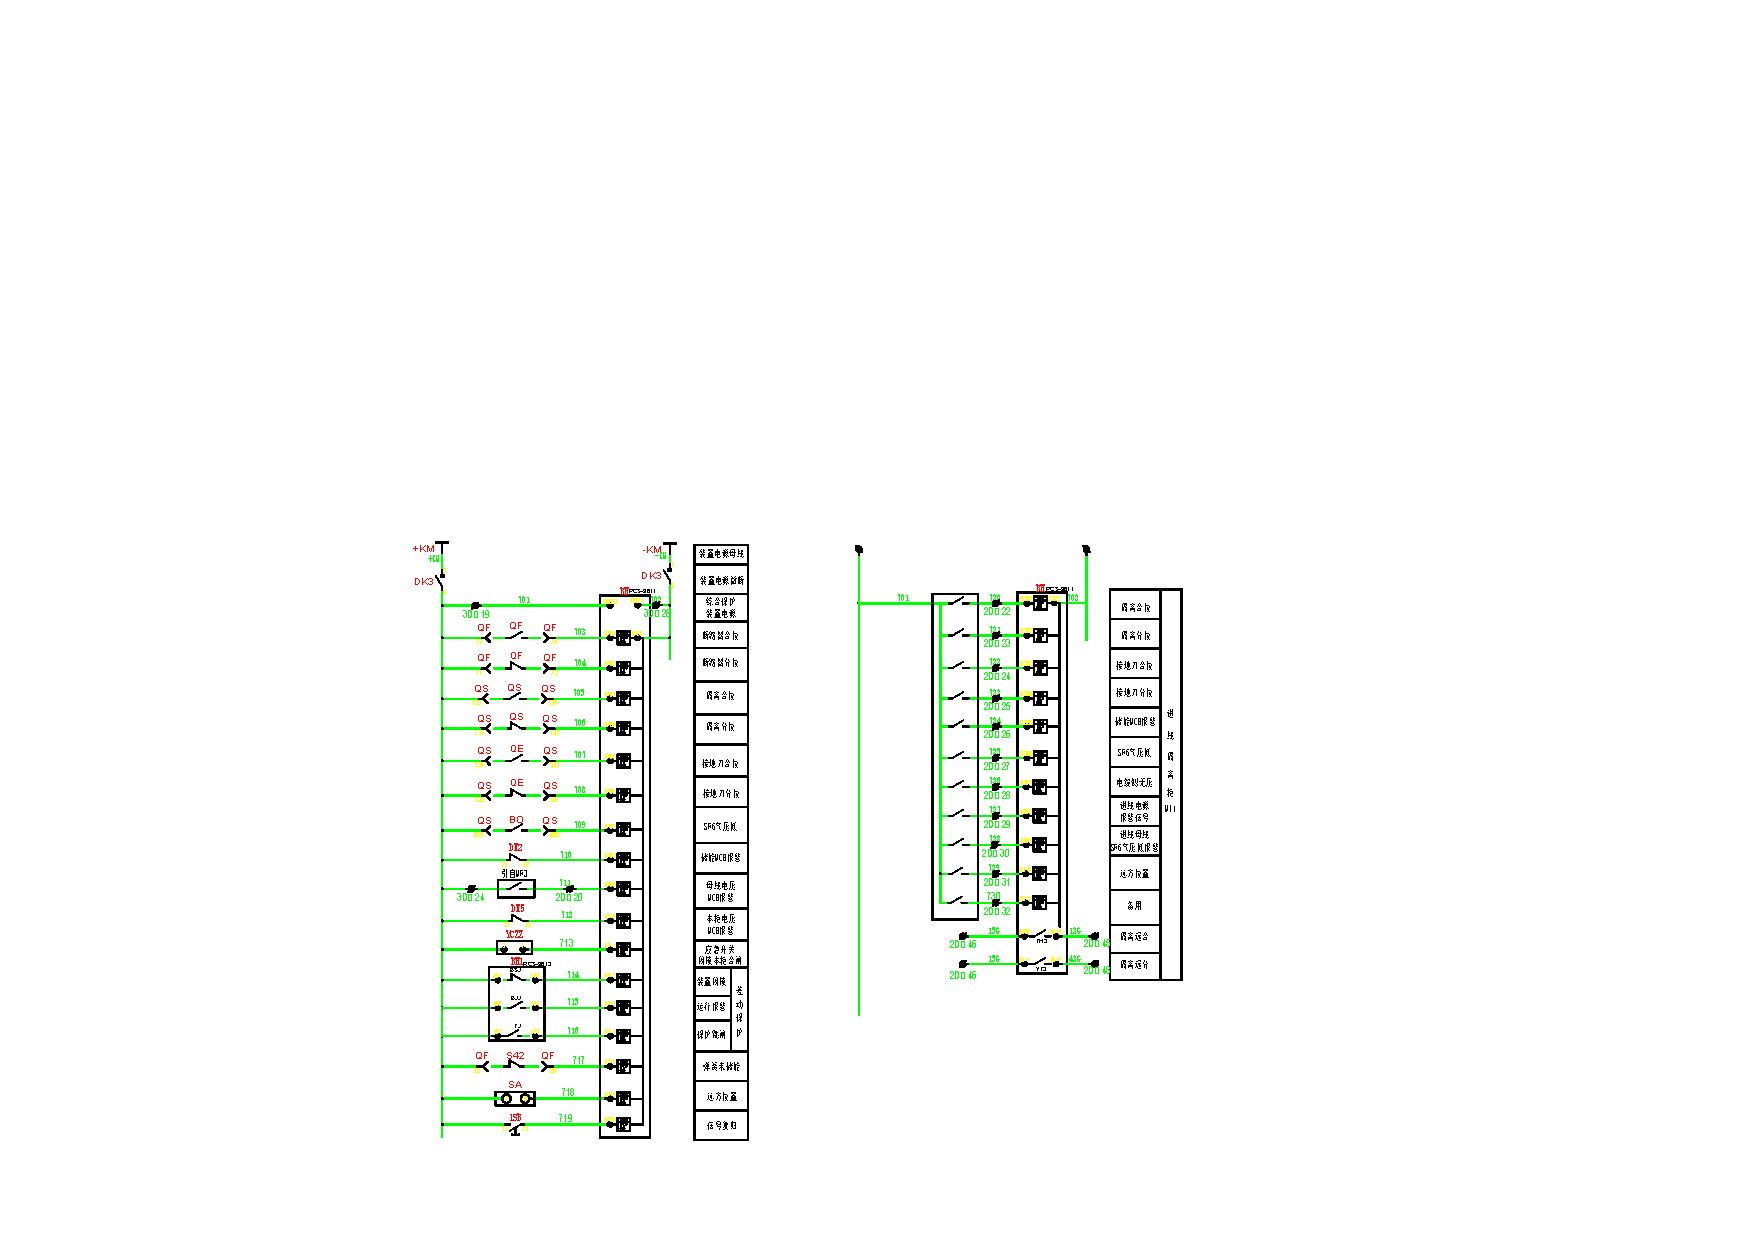
\includegraphics[width=0.6\textwidth]{进线柜控制回路图.pdf}
	\caption{进线柜控制回路图}
	\label{进线柜控制回路图}
\end{figure}

对进线柜不同的工作情况进行分析如下:

1. 遥控分闸:将SA打向“远方”位置,其内部接点“3”和“4”、“7”和“8”接通,将SA1打向分闸位,其内部接点“1”和“2”、“5”和“6”接通。此时电路路径如下:

$+KM$  $\Longrightarrow $    $BH0603-0604$  $\Longrightarrow $    $BH0804-0806$  $\Longrightarrow $    $QF14$  $\Longrightarrow $    $S16$  $\Longrightarrow $    $QF13$  $\Longrightarrow $    $QF20$(常开)   $\Longrightarrow $    合闸线圈   $\Longrightarrow $    $QF 21$  $\Longrightarrow $    $DK1$   $\Longrightarrow $    $-KM$接通,断路器分闸线圈受电,断路器断开,遥控分闸成功。

2. 遥控合闸:将SA打向“远方”位置,其内部接点“3”和“4”、“7”和“8”接通,将SA1打向合闸位,其内部接点“3”和“4”、“7”和“8”接通。此时电路路径如下:

$+KM$  $\Longrightarrow $    $BH0601-0602$  $\Longrightarrow $    $BH0810-0807$  $\Longrightarrow$    $QS514$  $\Longrightarrow$    $QE$(常开或常闭)  $\Longrightarrow $    $QS511$  $\Longrightarrow$    $QS114$或$QS113$ $\Longrightarrow$    $QS$(常开或常闭)  $\Longrightarrow $    $QS111$  $\Longrightarrow $    $QS812$  $\Longrightarrow $    $S24$  $\Longrightarrow $    $QS811$  $\Longrightarrow $    $BH0622-0621$  $\Longrightarrow $    $MCU17-16$  $\Longrightarrow $    常闭开关(引自$MI1$)  $\Longrightarrow $    常闭开关(引自$MM1$)  $\Longrightarrow $    $QF$  $\Longrightarrow $    $FTJ$  $\Longrightarrow $    合闸线圈  $\Longrightarrow $    $QF$  $\Longrightarrow $    $DK1$  $\Longrightarrow $    $-KM$接通,断路器合闸线圈受电,断路器闭合,遥控合闸成功。

3.手动分闸:将SA打向“就地”位置,其内部接点“1”和“2”、“5”和“6”接通,将SA1打向“分闸”位,其内部接点“1”和“2”、“5”和“6”接通。此时电路路径如下:

如\ref{进线柜控制回路图}中所示:$+KM$  $\Longrightarrow $    $DK1$  $\Longrightarrow $    $SA1-2$  $\Longrightarrow $    $SA11-2$  $\Longrightarrow $    $BH0804-0806$  $\Longrightarrow $    $QF14$  $\Longrightarrow $    $S16$  $\Longrightarrow $    $QF13$  $\Longrightarrow $    $QF20$(常开)  $\Longrightarrow $    合闸线圈  $\Longrightarrow $    $QF21$  $\Longrightarrow $    $DK1$  $\Longrightarrow $    $-KM$接通,断路器分闸线圈受电,断路器断开,手动分闸成功。

4.手动合闸:将SA打向“就地”位置,其内部接点“1”和“2”、“5”和“6”接通,将SA1打向“合闸”位,其内部接点“3”和“4”、“7”和“8”接通。此时电路路径如下:

如\ref{进线柜控制回路图}中所示:$+KM$  $\Longrightarrow $    $DK1$  $\Longrightarrow $    $SA1-2$  $\Longrightarrow $    $SA13-4$  $\Longrightarrow $    $BH0810-0807$  $\Longrightarrow $    $QS514$或$QS512$  $\Longrightarrow $    $QE$(常开或常闭合)  $\Longrightarrow $    $QS511$  $\Longrightarrow $    $QS114$或$QS113$  $\Longrightarrow $    $QS$(常开或常闭)  $\Longrightarrow $    $QS111$  $\Longrightarrow $    $QS812$  $\Longrightarrow $    $S24$  $\Longrightarrow $    $QS811$  $\Longrightarrow $    $BH0622-0621$  $\Longrightarrow $    $MCU17-16$  $\Longrightarrow $    常闭开关(引自$MI1$)  $\Longrightarrow $    常闭开关(引自$MM1$)  $\Longrightarrow $    $QF$  $\Longrightarrow $    $FTJ$  $\Longrightarrow $    合闸线圈  $\Longrightarrow $    $QF$  $\Longrightarrow $    $DK1$  $\Longrightarrow $    $-KM$接通,断路器合闸线圈受电,断路器闭合,手动合闸成功。

5. 遥分隔离:将SA打向“远方”位置,其内部接点“3”和“4”、“7”和“8”接通。此时电路路径如下:

如\ref{进线柜控制回路图}中所示:$+KM$  $\Longrightarrow $    $SA3-4$  $\Longrightarrow $    $BH0607-0608$  $\Longrightarrow $    $MCU11-15$  $\Longrightarrow $    $DK1$  $\Longrightarrow $    $-KM$接通,遥分隔离开关成功。

6. 遥合隔离:将SA打向“远方”位置,其内部接点“3”和“4”、“7”和“8”接通。此时电路路径如下:

如\ref{进线柜控制回路图}中所示:$+KM$  $\Longrightarrow $    $SA3-4$  $\Longrightarrow $    $BH0605-0606$  $\Longrightarrow $    常闭开关(引自分段柜母线未接地)  $\Longrightarrow $    $MCU10-15$  $\Longrightarrow $    $DK1$  $\Longrightarrow $    $-KM$接通,遥合隔离开关成功。

7.手分隔离:将SA打向“就地”位置,其内部接点“1”和“2”、“5”和“6”接通,将SA2打向“分闸”位,其内部接点“1”和“2”、“5”和“6”接通。此时电路路径如下:

如\ref{进线柜控制回路图}中所示:$+KM$  $\Longrightarrow $    $DK1$  $\Longrightarrow $    $SA1-2$  $\Longrightarrow $    $SA21-2$  $\Longrightarrow $    $MCU11-15$  $\Longrightarrow $    $DK1$  $\Longrightarrow $    $-KM$接通,手分隔离成功。

8.手合隔离:将SA打向“就地”位置,其内部接点“1”和“2”、“5”和“6”接通,将SA2打向“合闸”位,其内部接点“3”和“4”、“7”和“8”接通。此时电路路径如下:

如\ref{进线柜控制回路图}中所示:$+KM$  $\Longrightarrow $    $DK1$  $\Longrightarrow $    $SA1-2$  $\Longrightarrow $    $SA23-4$  $\Longrightarrow $    常闭开关(引自分段柜母线未接地)  $\Longrightarrow $    $MCU10-15$  $\Longrightarrow $    $DK1$  $\Longrightarrow $    $-KM$接通,手合隔离开关成功。

9. 手分地刀:将SA打向“就地”位置,其内部接点“1”和“2”、“5”和“6”接通,将SA3打向分闸位,接点“1”和“2”、“5”和“6”接通。此时电路路径如下:

如\ref{进线柜控制回路图}中所示:$+KM$  $\Longrightarrow $    $SA1-2$  $\Longrightarrow $    $SA31-2$  $\Longrightarrow $    $MCU13-15$  $\Longrightarrow $    $DK1$  $\Longrightarrow $    $-KM$接通,手分隔离地刀成功。

10. 手合地刀:将SA打向“就地”位置,其内部接点“1”和“2”、“5”和“6”接通,将SA3打向合闸位,接点“3”和“4”、“7”和“8”接通。此时电路路径如下:

如\ref{进线柜控制回路图}中所示:$+KM$  $\Longrightarrow $    $SA1-2$  $\Longrightarrow $    $SA33-4$  $\Longrightarrow $    $MCU12-15$  $\Longrightarrow $    $DK1$  $\Longrightarrow $    $-KM$接通,手合隔离地刀成功。

这些情况描述了不同的工作状态和对应的电路路径。其中的“+KM”和“-KM”表示正负电源信号,其他元件也在电路中扮演着不同的角色。

\subsection{进线柜交流和测量回路分析}
进线柜交流和测量回路图如\ref{进线柜交流和测量回路图}所示:
\begin{figure}[h]
	\centering
	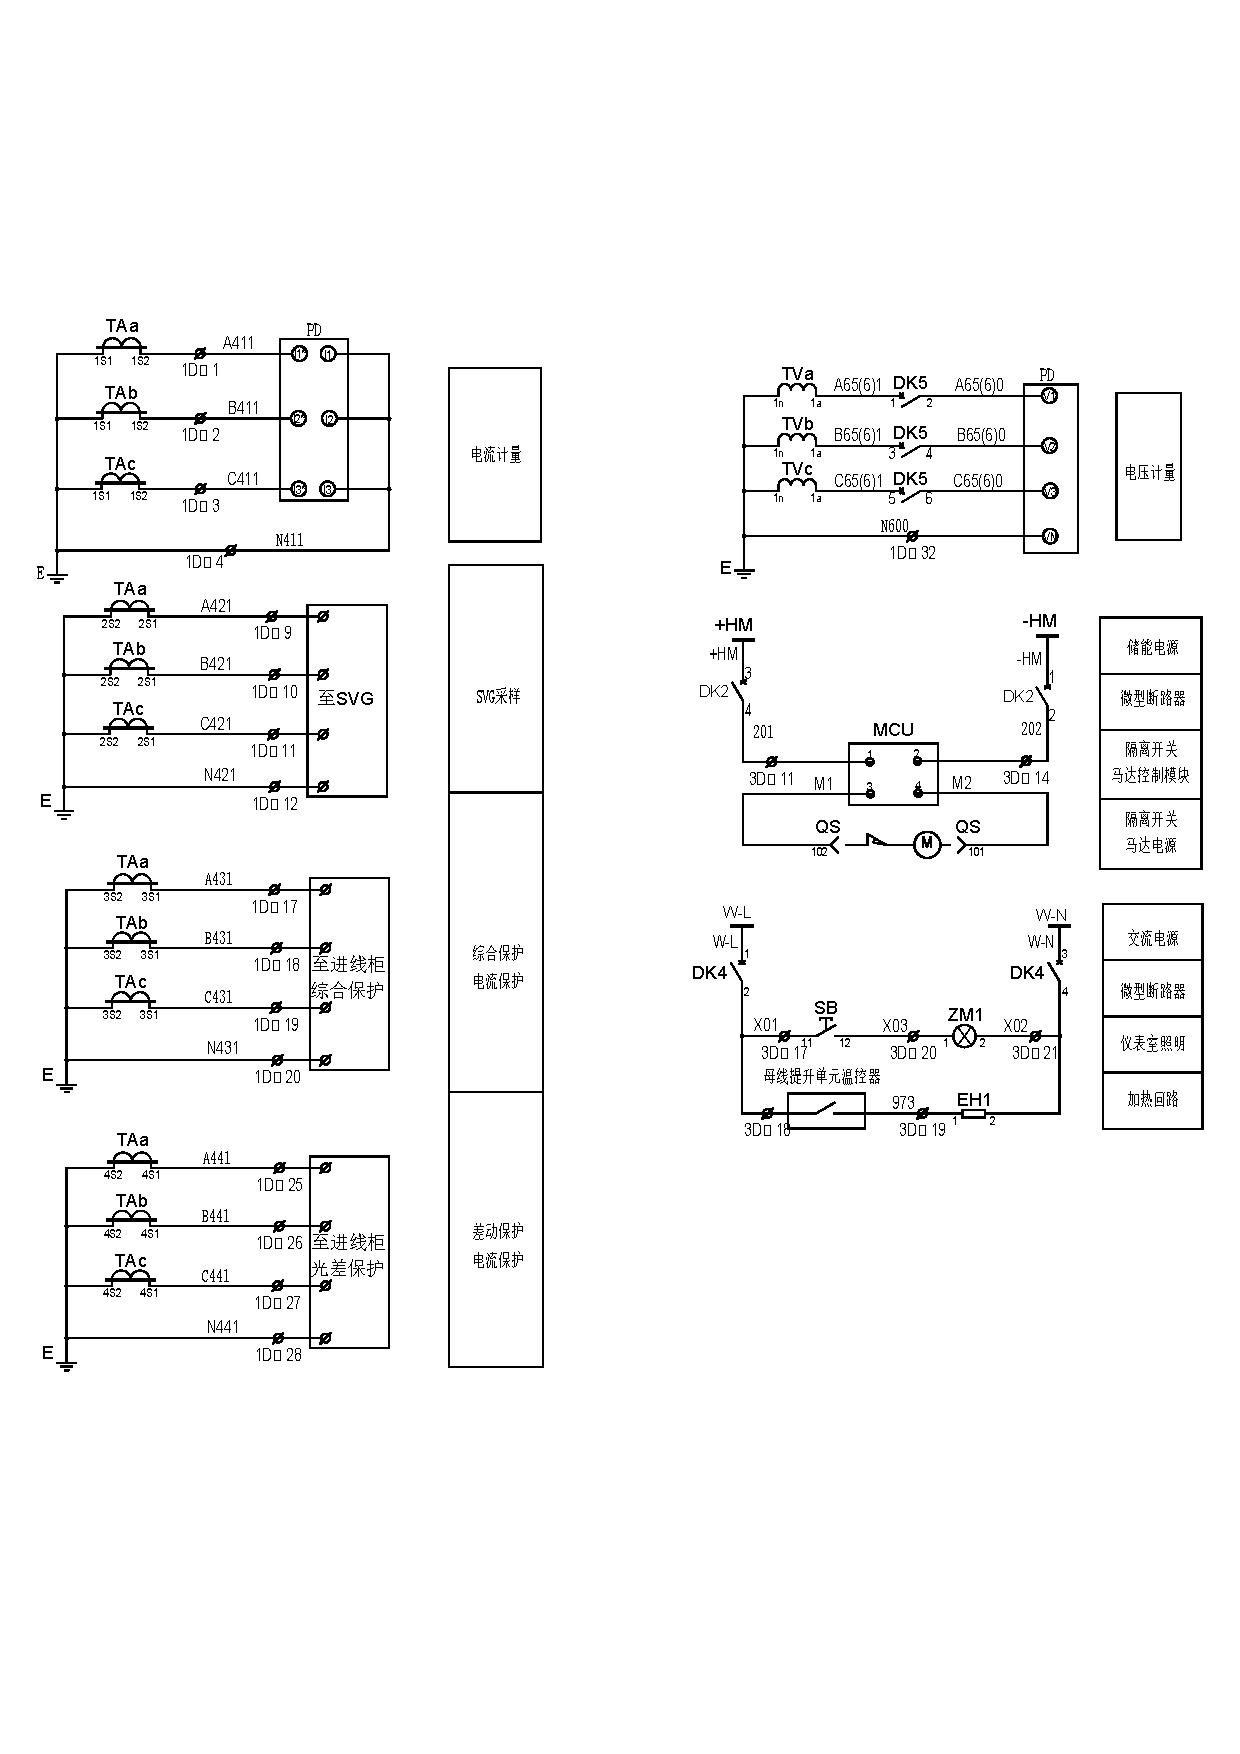
\includegraphics[width=0.6\textwidth]{进线柜交流和测量回路图.pdf}
	\caption{进线柜交流和测量回路图}
	\label{进线柜交流和测量回路图}
\end{figure}
根据所学内容,交流回路可以分为电压回路和电流回路。在上图中,1\#进线柜的交流回路包括综合电流保护回路、差动电流保护回路、母线电压保护测量回路和母线电压差动保护测量回路。其中,后两个电路还具有测量功能。

在这四个电路中,与电流相关的交流测量回路,如综合电流保护回路和差动电流保护回路,其电源来自计量柜相应的电流互感器的二次侧。而与电压相关的交流测量回路,如母线电压保护测量回路和母线电压差动保护测量回路,其电源来自计量柜相应的电压互感器的二次侧。一旦获取了相应的电压和电流信息,这些信息通过各自的电路连接,然后反馈给相应的回路,以实现测量和保护功能。

\section{计量柜二次接线图分析}

在城轨供变电技术中,计量柜的主要作用是监测、测量和记录电能的使用情况,以支持电费计算、能源管理、负荷分析、故障检测、合规性以及能源节约。这有助于确保城轨系统的可靠供电、经济运营和可持续性。

计量柜用于测量和记录城轨系统中所消耗的电能,以确保准确的电能计量和记录,从而进行电费计算和能源管理。通常,计量柜包括电能表(电表)和其他测量设备,用于测量电能的消耗。通过计量柜,城轨运营商能够监测电能的使用情况,分析负荷曲线,辨识高峰和低谷负荷时段,以更好地规划供电和能源采购策略。这有助于提高电力系统的效率并降低运营成本。

\subsection{计量柜控制信号回路分析}
计量柜控制信号回路图如\ref{进线柜控制回路图}所示:

\begin{figure}[h]
	\centering
	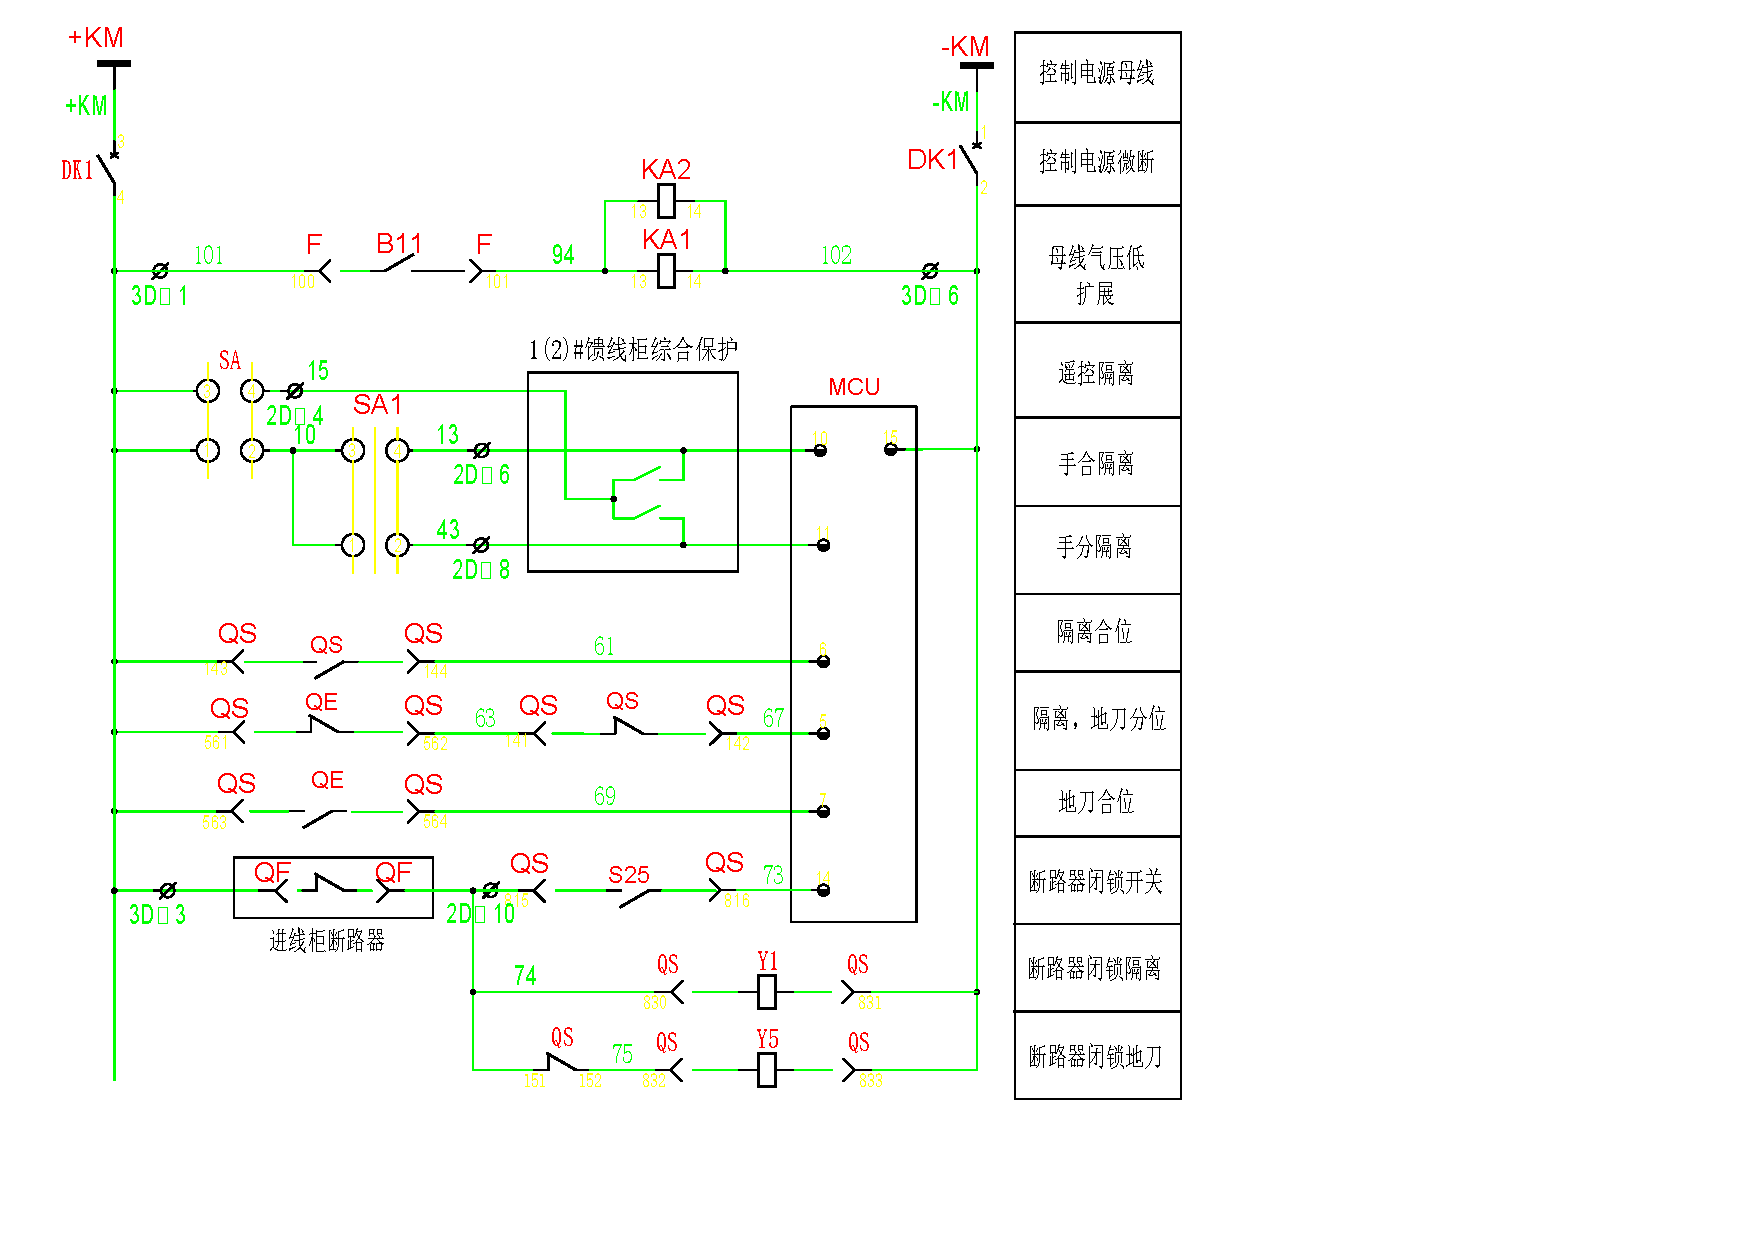
\includegraphics[width=0.6\textwidth]{计量柜控制信号回路图.pdf}
	\caption{计量柜控制信号回路图}
	\label{计量柜控制信号回路图}
\end{figure}

1. 手动分隔离开关:将远方就地控制开关SA打到"就地"位置,接通1-2和5-6接点。然后将隔离控制开关SA1打到"分闸"位置,接通1-2和5-6接点。电路路径为$+KM$ $\Longrightarrow $ $DK1$ $\Longrightarrow $ $SA1-2$ $\Longrightarrow $ $SA11-2$ $\Longrightarrow $ $MCU11-15$ $\Longrightarrow $ $DK1$ $\Longrightarrow $ $-KM$接通,实现手动分隔离开关功能。

2. 手动合隔离开关:将远方就地控制开关SA打到"就地"位置,接通1-2和5-6接点。然后将隔离控制开关SA1打到"合闸"位置,接通3-4和7-8接点。电路路径为$+KM$ $\Longrightarrow $ $DK1$ $\Longrightarrow $ $SA1-2$ $\Longrightarrow $ $SA13-4$ $\Longrightarrow $ $MCU10-15$ $\Longrightarrow $ $DK1$ $\Longrightarrow $ $-KM$接通,实现手动合隔离开关功能。

3. 遥控分隔离开关:将远方就地控制开关SA打到"远方"位置,接通3-4和7-8接点。电路路径为$+KM$ $\Longrightarrow $ $DK1$ $\Longrightarrow $ $SA3-4$ $\Longrightarrow $ 进线柜综合保护 $\Longrightarrow $ $MCU11-15$ $\Longrightarrow $ $DK1$ $\Longrightarrow $ $-KM$接通,实现遥控分隔离开关功能。

4. 遥控合隔离开关:将远方就地控制开关SA打到"远方"位置,接通3-4和7-8接点。电路路径为$+KM$ $\Longrightarrow $ $DK1$ $\Longrightarrow $ $SA3-4$ $\Longrightarrow $ 进线柜综合保护 $\Longrightarrow $ $MCU10-15$ $\Longrightarrow $ $DK1$ $\Longrightarrow $ $-KM$接通,实现遥控合隔离开关功能。

5. 断路器闭锁:当与QF合作使用的隔离开关采用电气控制操作机构时,要求在QF处于分闸位置时才能进行QS的任何操作。当QF处于分闸状态时,其进线柜断路器的常闭接点闭合。电路路径为$+KM$ $\Longrightarrow $ $DK1$ $\Longrightarrow $ 进线柜断路器 $\Longrightarrow $ $S25$ $\Longrightarrow $ $MCU14-15$ $\Longrightarrow $ $DK1$ $\Longrightarrow $ $-KM$接通,实现断路器闭锁功能。

\subsection{计量柜交流和测量回路信号分析}

计量柜的二次回路主要包括电流计量、电压计量、差动电流保护、综合电流保护以及SVG采样五个部分。下面对这五个部分的工作原理进行分析。

1. 电流计量:

\begin{figure}[h]
	\centering
	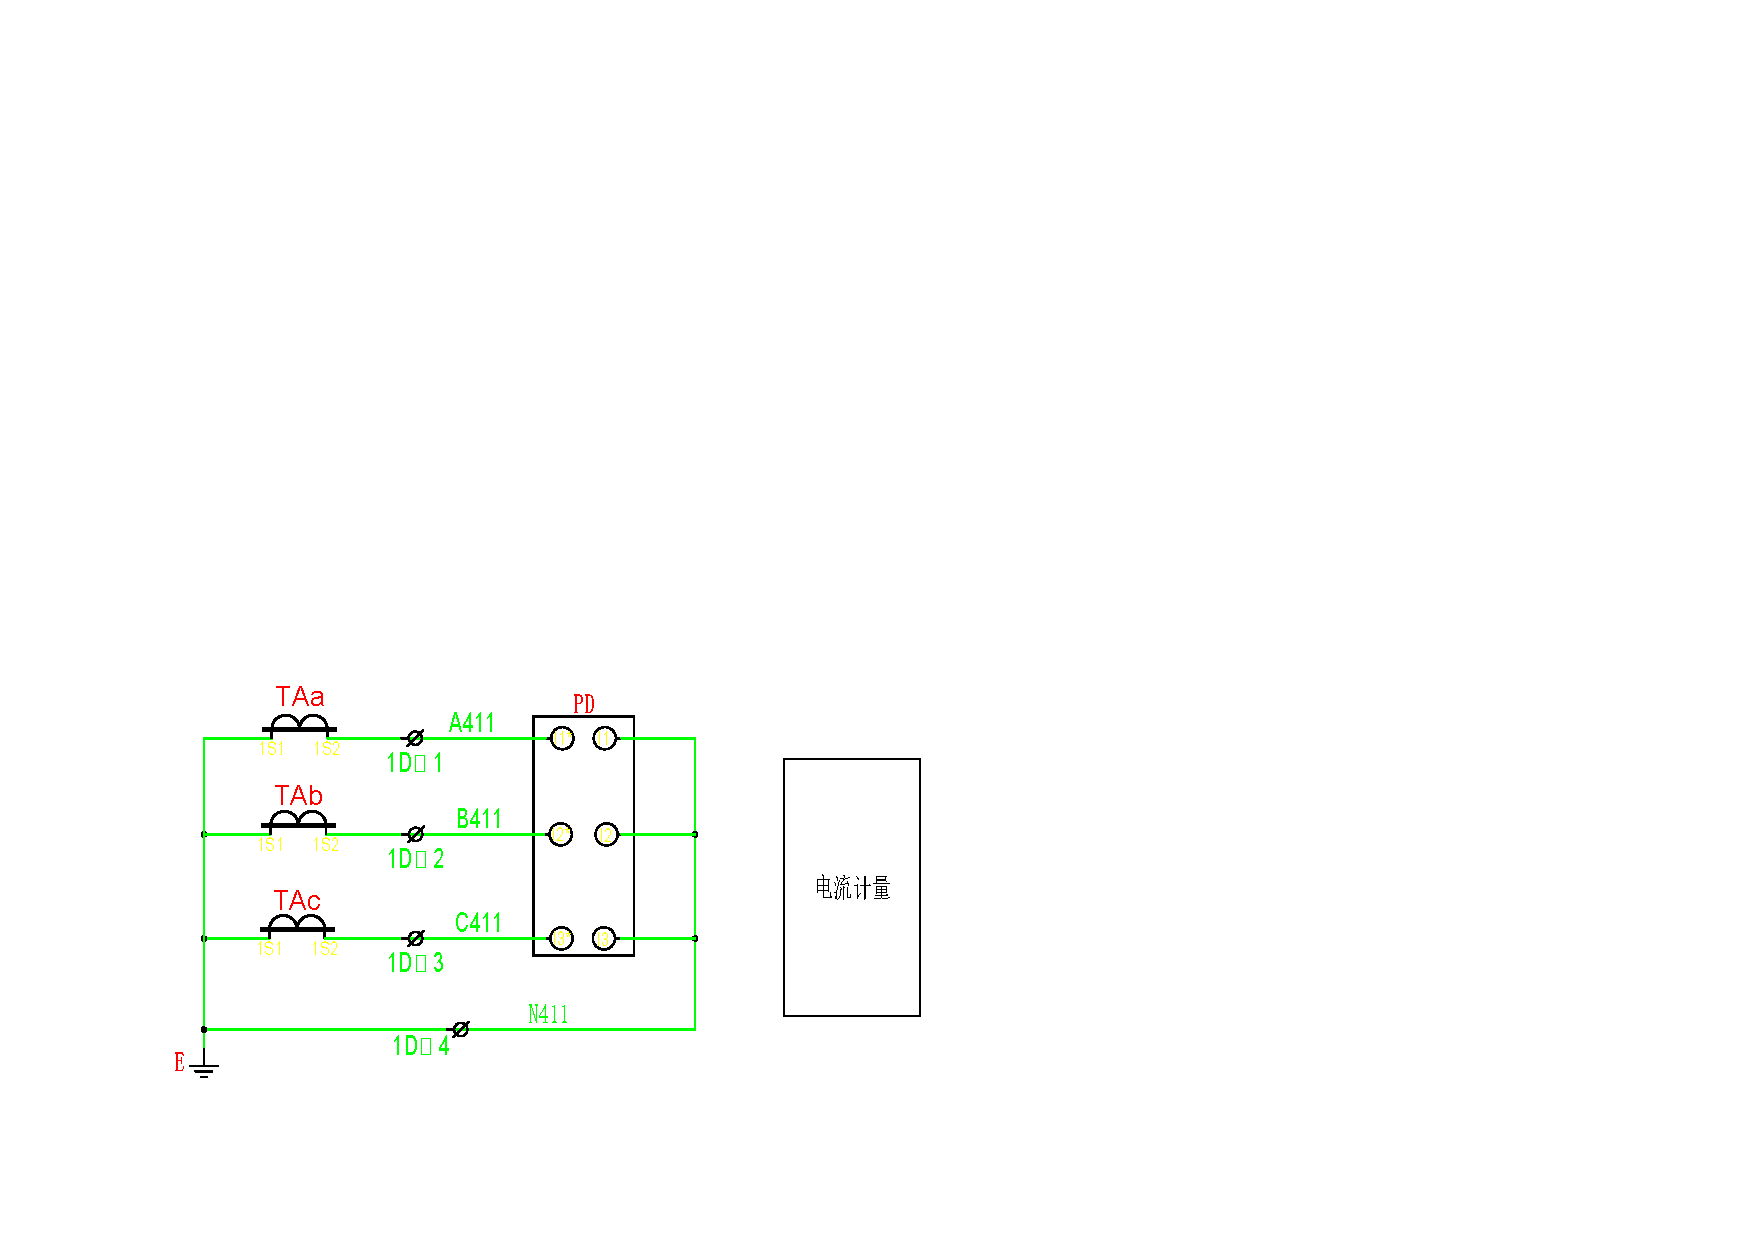
\includegraphics[width=0.6\textwidth]{电流计量.pdf}
	\caption{电流计量}
	\label{电流计量}
\end{figure}

电流计量部分用于测量电流的消耗。它通常包括电流互感器和电流计量装置。电流互感器将一次侧电流转换为二次侧电流,然后电流计量装置测量并记录二次侧电流的数值。这样可以准确测量电流的消耗情况,用于电能计量和能源管理。

2. 电压计量:

\begin{figure}[h]
	\centering
	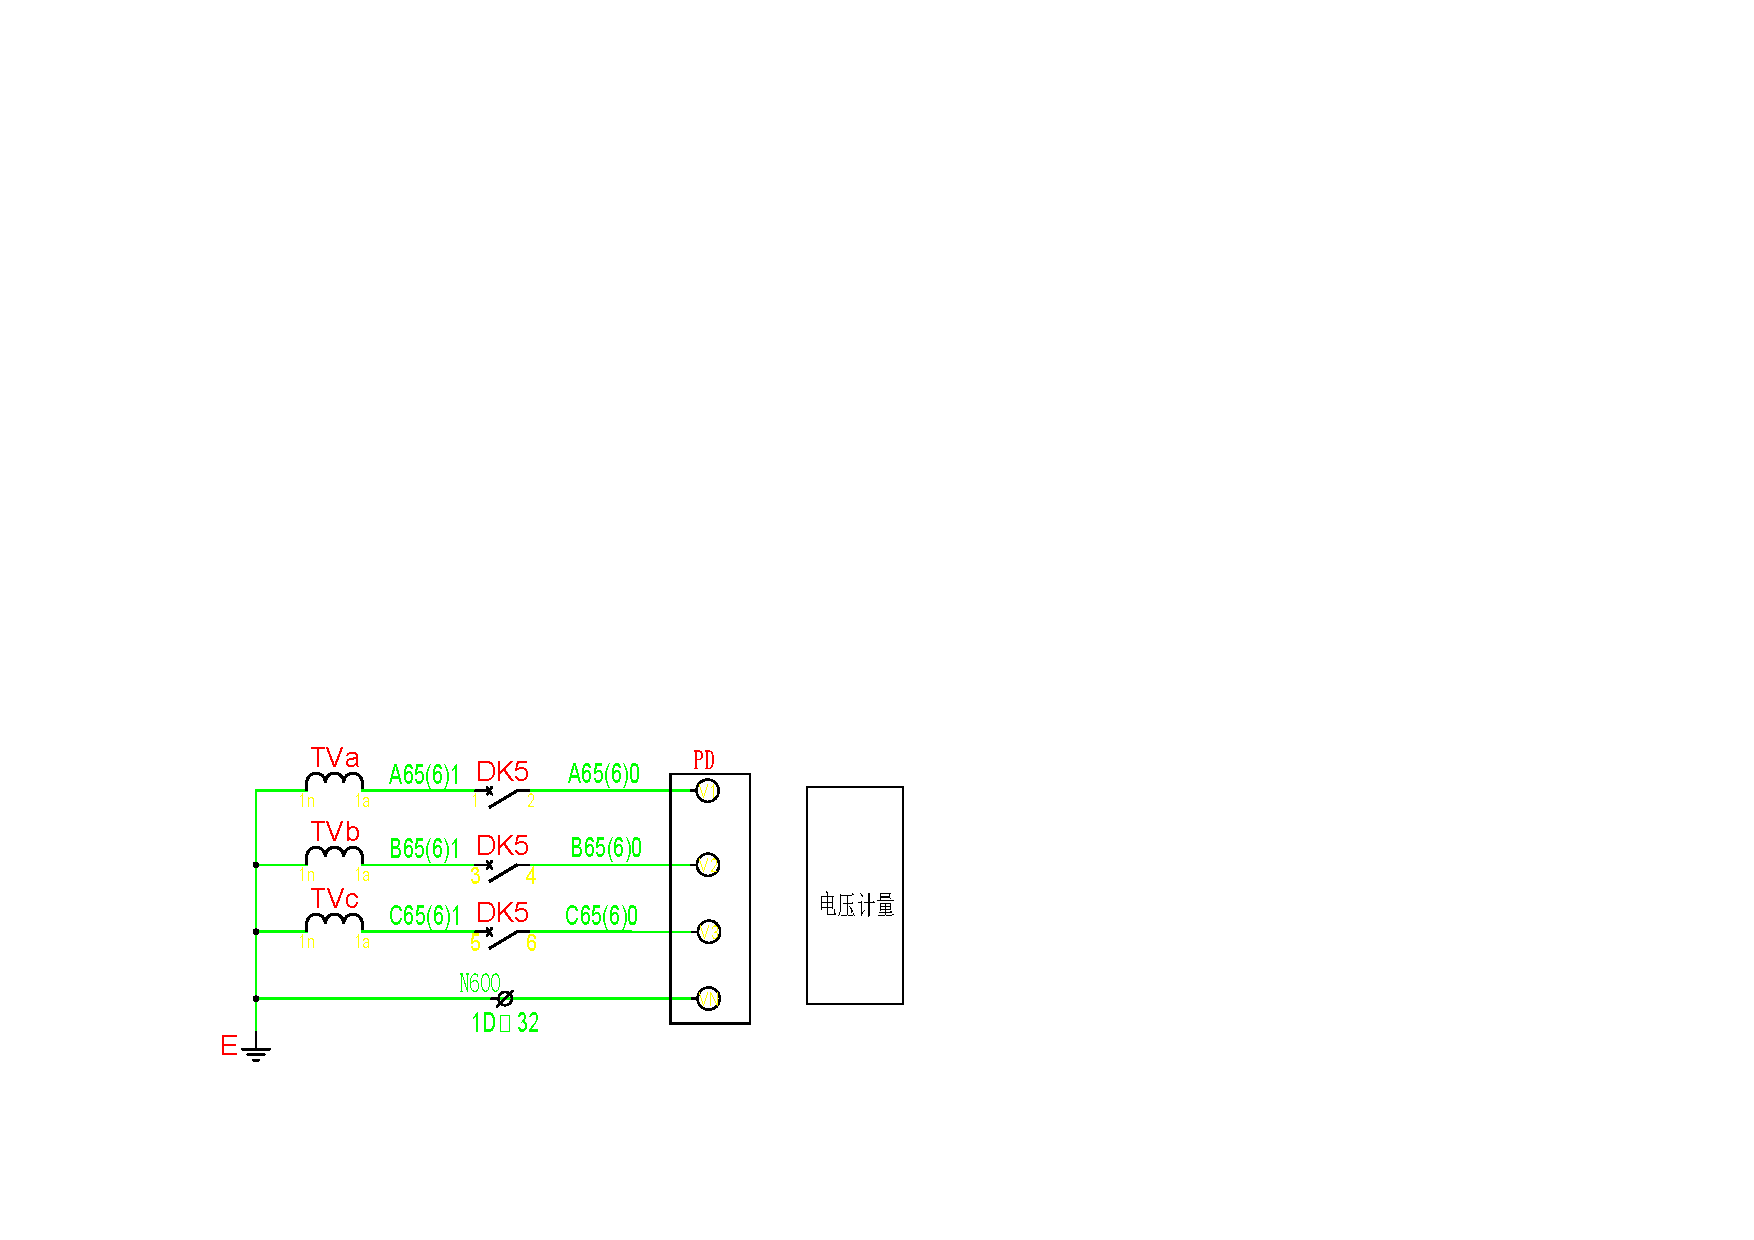
\includegraphics[width=0.6\textwidth]{电压计量.pdf}
	\caption{电压计量}
	\label{电压计量}
\end{figure}

电压计量部分用于测量电压的数值。它包括电压互感器和电压计量装置。电压互感器将一次侧电压转换为二次侧电压,然后电压计量装置测量并记录二次侧电压的数值。这有助于准确测量电压的消耗情况,用于电能计量和能源管理。

3. 差动电流保护:

\begin{figure}[h]
	\centering
	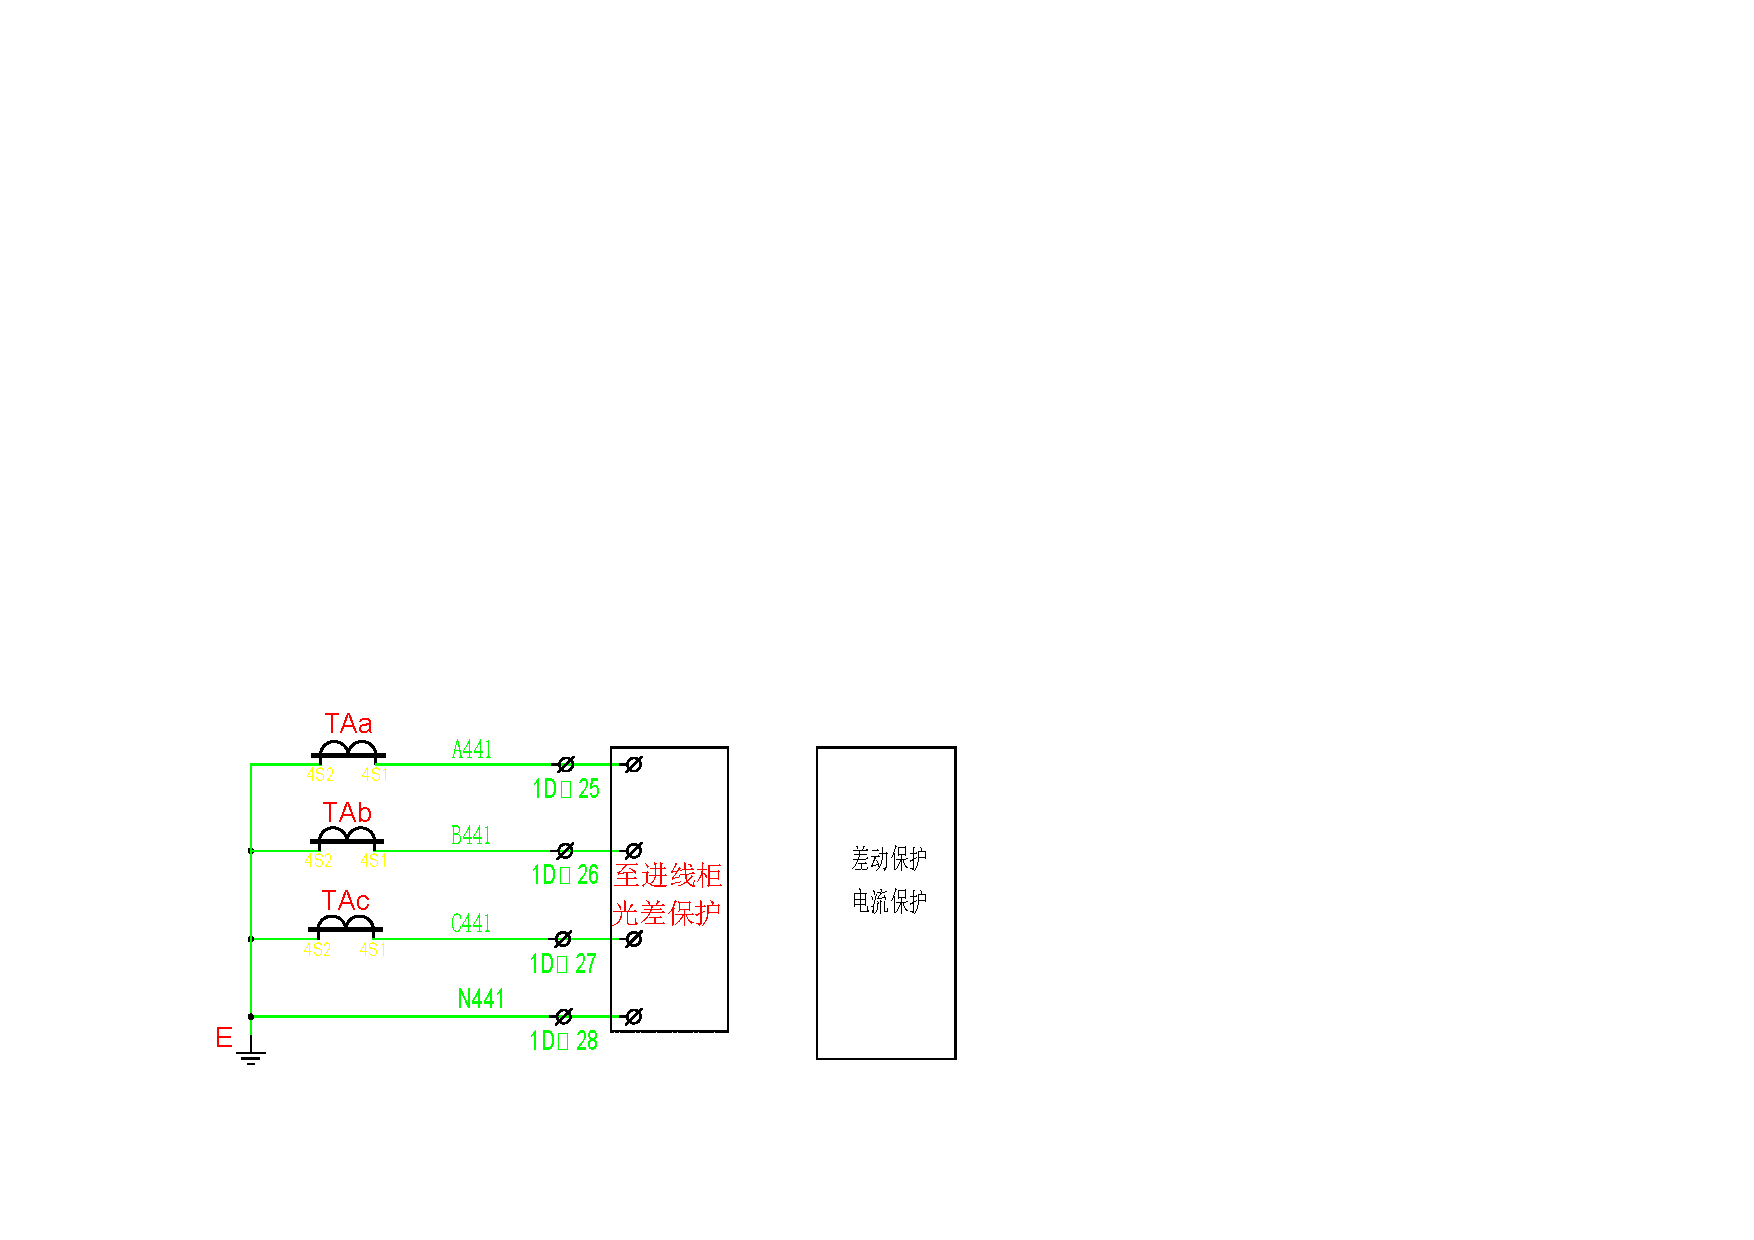
\includegraphics[width=0.6\textwidth]{差动电流保护.pdf}
	\caption{差动电流保护}
	\label{差动电流保护}
\end{figure}

差动电流保护部分用于检测系统中的电流差异。它通常包括差动电流互感器和差动电流保护装置。差动电流互感器测量一次侧电流的总和,并与二次侧电流的总和进行比较。如果两者不相等,说明系统中存在电流差异,可能发生故障。差动电流保护装置会触发保护动作以隔离故障。
\newpage
4. 综合电流保护:

\begin{figure}[h]
	\centering
	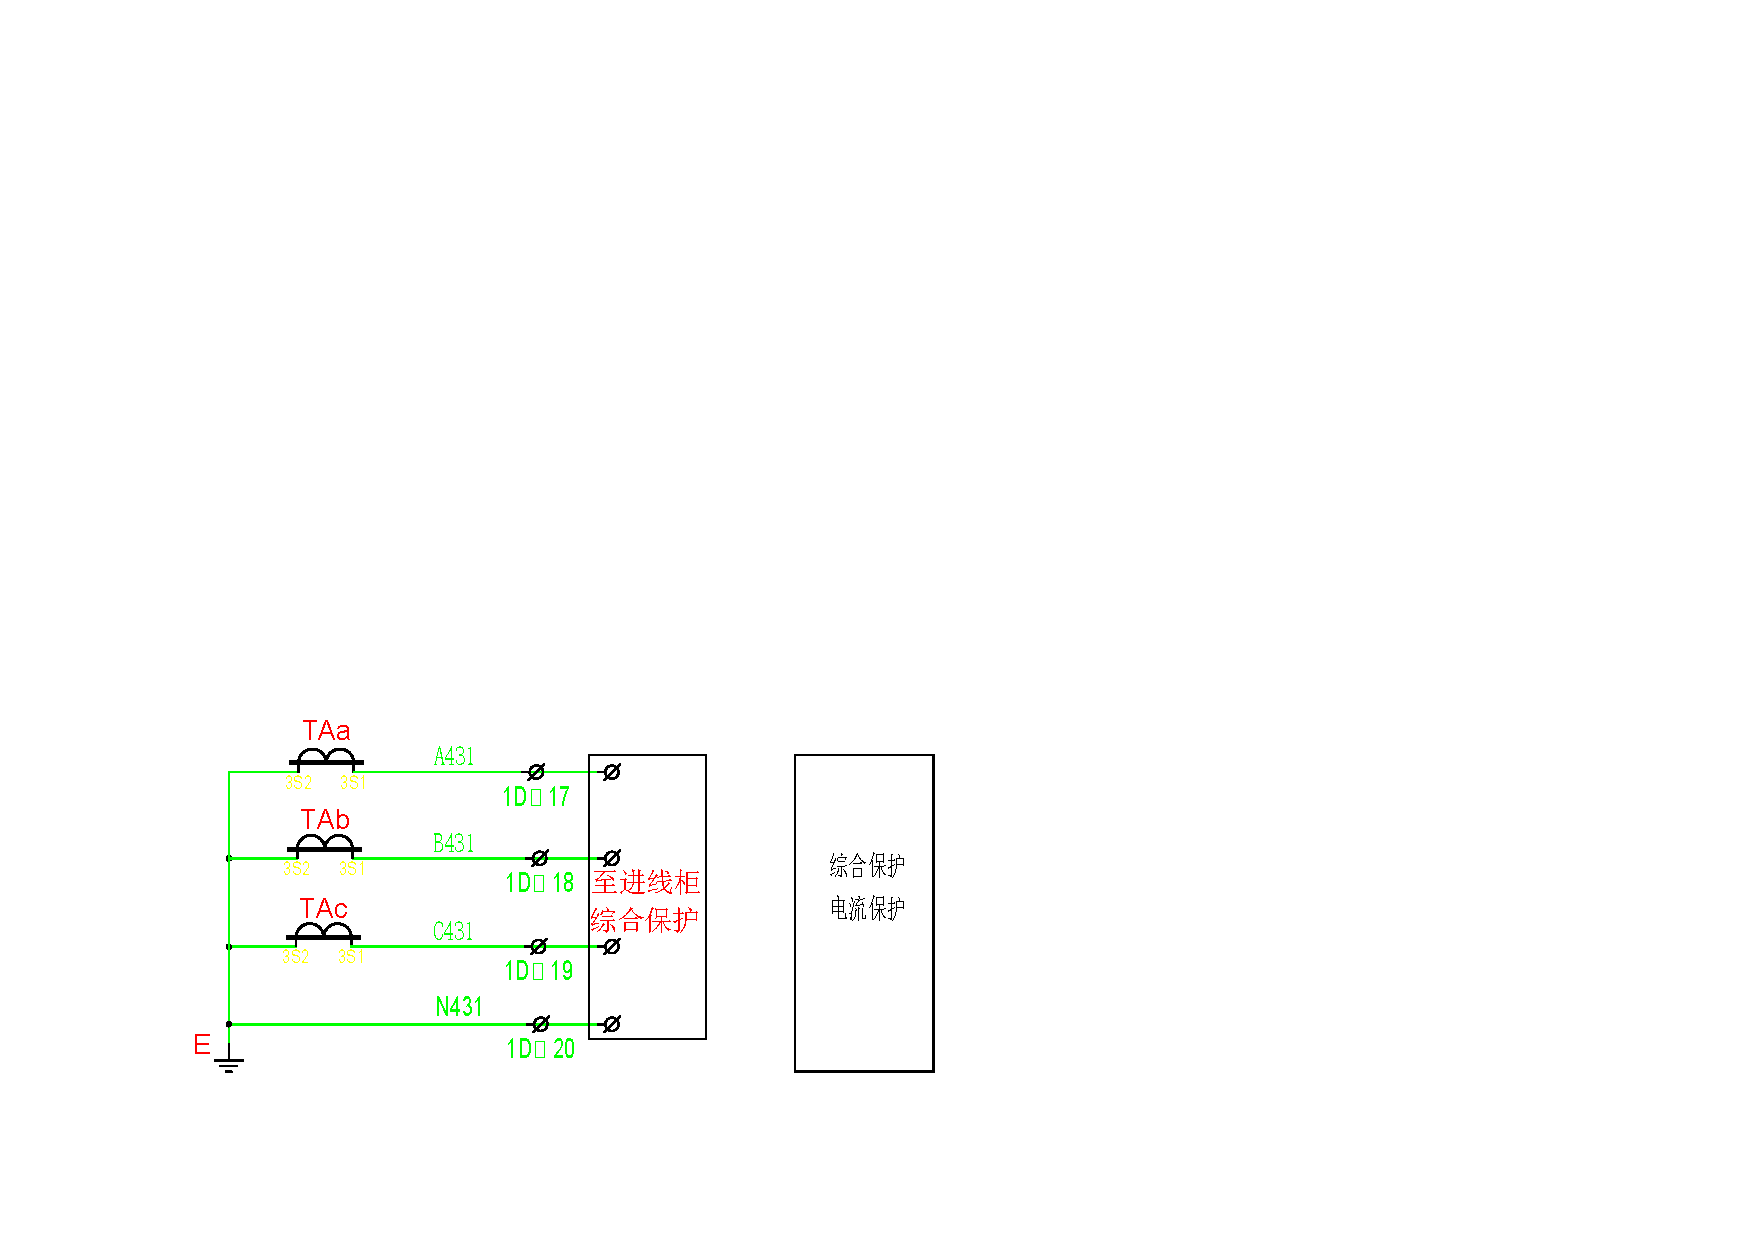
\includegraphics[width=0.6\textwidth]{综合保护电流保护.pdf}
	\caption{综合保护电流保护}
	\label{综合保护电流保护}
\end{figure}

综合电流保护部分用于保护电力系统免受电流异常情况的影响。它通常包括综合电流互感器和综合电流保护装置。综合电流互感器测量一次侧电流的总和,并将数据传递给综合电流保护装置。如果电流异常超过设定的阈值,综合电流保护装置将触发保护操作以防止系统受到损害。

5. SVG采样:

\begin{figure}[h]
	\centering
	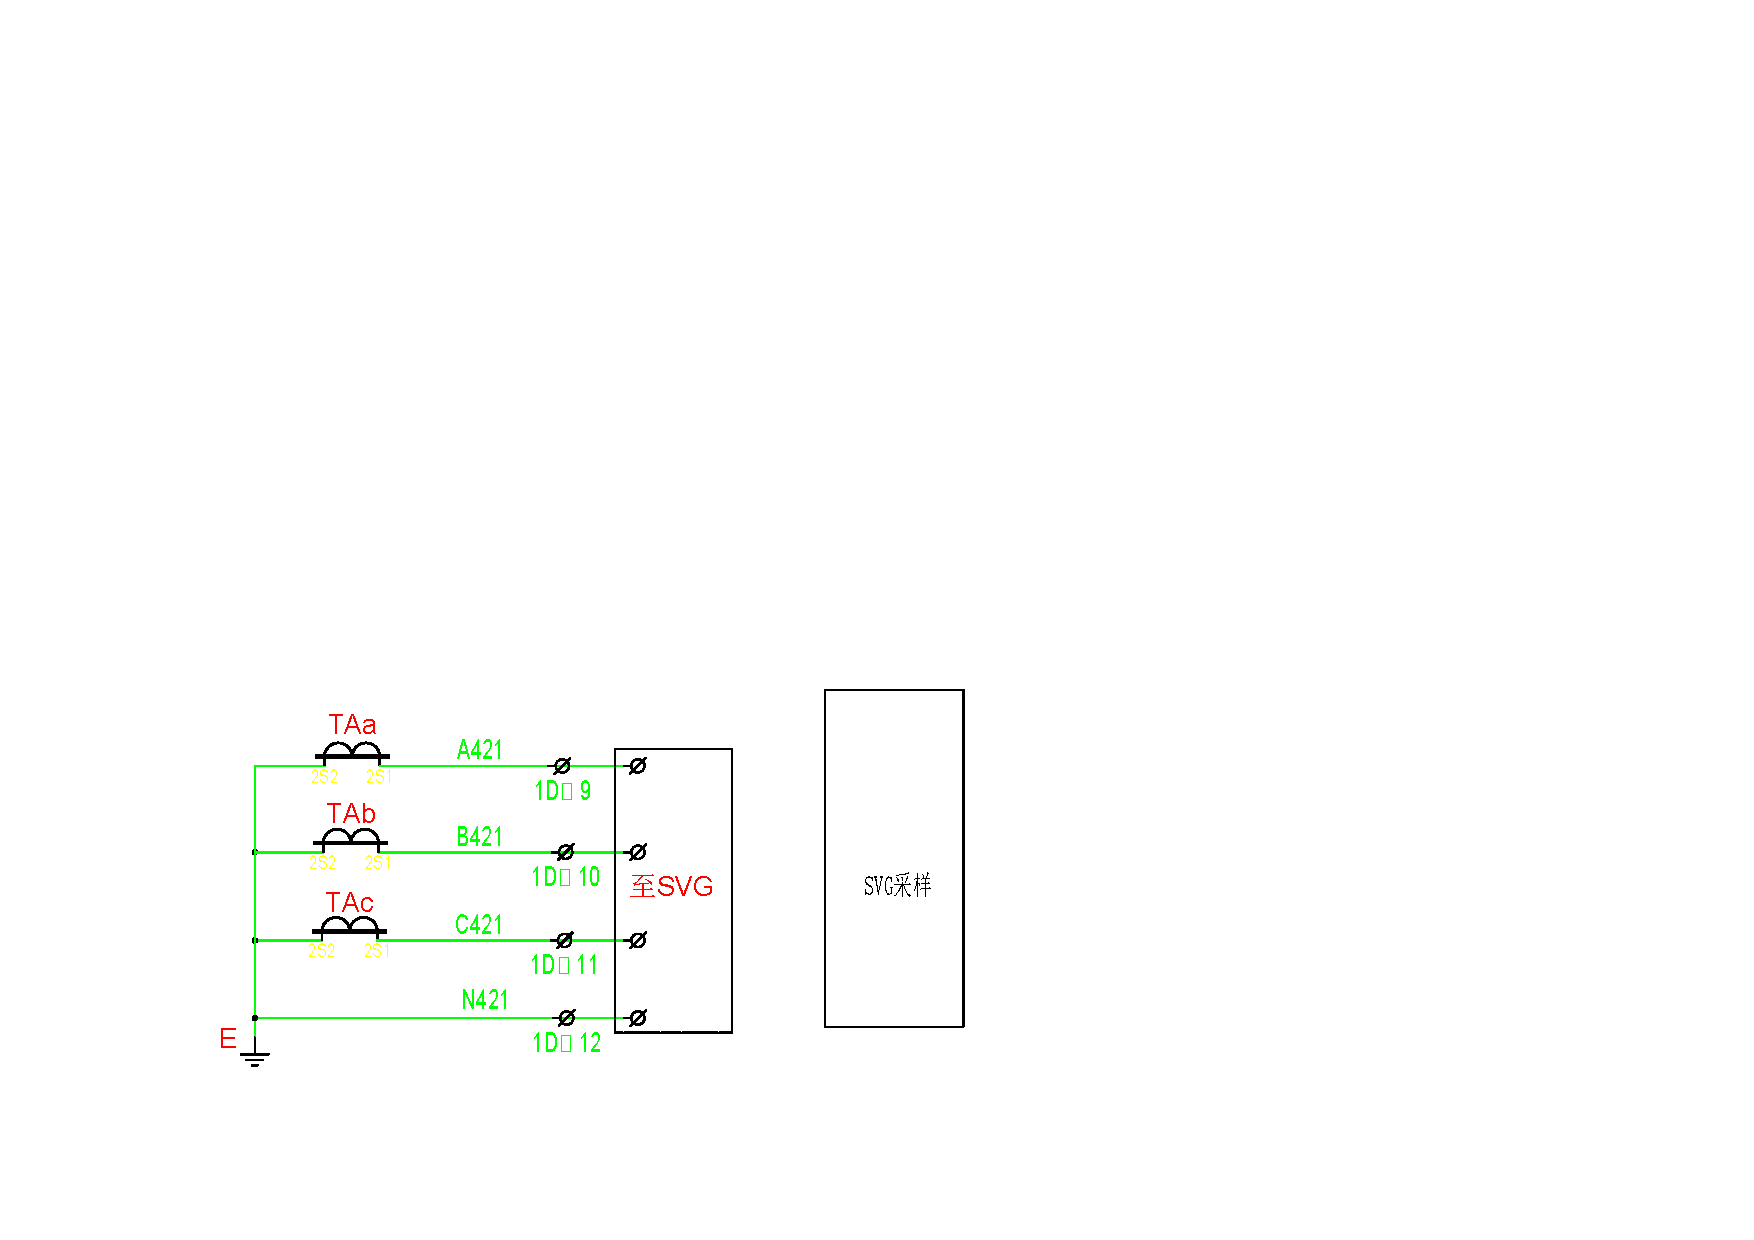
\includegraphics[width=0.6\textwidth]{SVG采样.pdf}
	\caption{SVG采样}
	\label{SVG采样}
\end{figure}

SVG采样部分用于采集数据并提供给SVG(Static Var Generator,静止有功功率发生器)。这有助于SVG根据系统需求调整电流,以维持电压和无功功率的稳定性。通过采样和数据传递,SVG可以有效地管理电力系统的无功功率流动,以提高系统性能。

这些部分共同工作,确保计量柜能够准确测量和记录电能的使用情况,以支持电费计算、能源管理和系统保护。

\section{总结}
本章主要关注青岛-海阳城际轨道交通工程施工设计原始资料图中的二次接线图部分,重点分析1\#进线柜和计量柜的控制信号回路、交流回路、测量回路,并详细研究它们各个功能的具体实现原理。

对于1\#进线柜的控制信号回路,特别关注遥控分/合闸、手动分/合闸、遥分/合隔离、手分/合隔离、手分/合地刀的具体实现方式,以及列举出各功能中的具体二次接线回路。同时,对交流和测量回路进行详细分析,包括综合电流保护回路、差动电流保护回路、母线电压保护测量回路、母线电压差动保护测量回路的电路构成和电压电流的来源,以及保护测量的大致原理。

对于计量柜的控制信号回路,着重分析手动分/合隔离开关、遥控分/合隔离开关、断路器闭锁的具体实现方式,并列举构成这些功能的二次接线回路。其他功能的实现与1\#进线柜类似,此处不再赘述。另外,对交流和测量回路进行详细研究,包括电流计量、电压计量、差动电流保护、综合电流保护、SVG采样的电路构成以及实现保护测量的大致原理。

这些分析有助于更深入地理解这些关键部分的工作原理,以确保城际轨道交通工程施工设计的可靠性和正常运行。

